\documentclass[DIV=14]{scrarticle}
\usepackage[utf8]{inputenc}
\usepackage[T1]{fontenc}  % needed for the correct underscores in \texttt
\usepackage{graphicx}
\usepackage{amsmath}

\usepackage{siunitx}
\DeclareSIUnit{\LSB}{LSB}

\usepackage{hyperref}
\hypersetup{pdfborder = 0 0 0}  % links without decoration

\usepackage{censor} % just for the sample report, no use in a real report

\titlehead{
    Laboratory for Electrical Instrumentation and Embedded Systems \\
    IMTEK -- Department of Microsystems Engineering \\
    University of Freiburg \vspace{0.5cm} \\ 
    Sensors Lab Course \\   
    Winter term 2022/23 \vspace{1.5cm}}

\title{Lab Report M1}
\subtitle{Gyroscope and Acceleration Sensors} 
\author{Rafael Andrioli Bauer (5163344)}

\begin{document}



\maketitle

\thispagestyle{empty}

\vfill
\begin{center}
    
\includegraphics{ufcd-logo-e1-a4-color.pdf} \vspace{1cm} \\ 
\end{center}
\vfill

% Comment out the entire 'flushleft' block if you did the experiments alone
\begin{flushleft}
Data generated in a team together with
\begin{itemize}
    \item Robert Hooke (2718281)
    \item Edmond Halley (1414213)
\end{itemize}
\end{flushleft}



\clearpage

\section{Introduction}

Rotating or swinging systems have fascinated us since childhood. On most children’s playgrounds we have swings and merry-go-rounds. In this module, the accelerometer and gyroscope of the Nicla Sense ME Board were investigated on a merry-go-round linking the radial acceleration and rotational velocity together. Before, the gyroscope gets characterized for offset and noise. \cite{labManual}

\section{Theory}
In a rotating frame of reference, the centrifugal force appears as an inertial force (“fictitious force”), pulling objects outwards from the center of rotation. The centripetal force from Newtonian mechanics is in a circular motion pointing towards the center of rotation and thus opposing the centrifugal force. Written as centripetal acceleration $a_\mathrm{c}$, it depends on the radius $r$ and the square of the rotational velocity $\mathit{\Omega}$ and is accordingly independent of the rotational direction:
\begin{equation}
    a_\mathrm{c} = r\, \mathit{\Omega}^2
\end{equation}
The rotational velocity $\mathit{\Omega}$ must be in \si{\radian\per\second} to comply with the SI units.


\subsection{Gyroscope}
In a gyroscope, the Coriolis effect provides the principle to translate rotational velocity with the help of a linear motion to a detectable effect. The Coriolis force ($\boldsymbol{F}_\mathrm{c}$) is proportional to the cross product of the linear motion ($\boldsymbol{v}$) of the moving object with mass $m$ and the rotational velocity vector ($\boldsymbol{\mathit{\Omega}}$):
\begin{equation}
    \boldsymbol{F}_\mathrm{c} = 2m (\boldsymbol{v} \times \boldsymbol{\mathit{\Omega}}) 
\end{equation}

Microfabricated gyroscopes use an oscillating linear motion and detect the corresponding orthogonal displacement caused by the Coriolis force. Figure~\ref{fig:gyroscope} illustrates a typical sensor setup. 

\vspace{1em}

\begin{figure}[h]
    \centering
    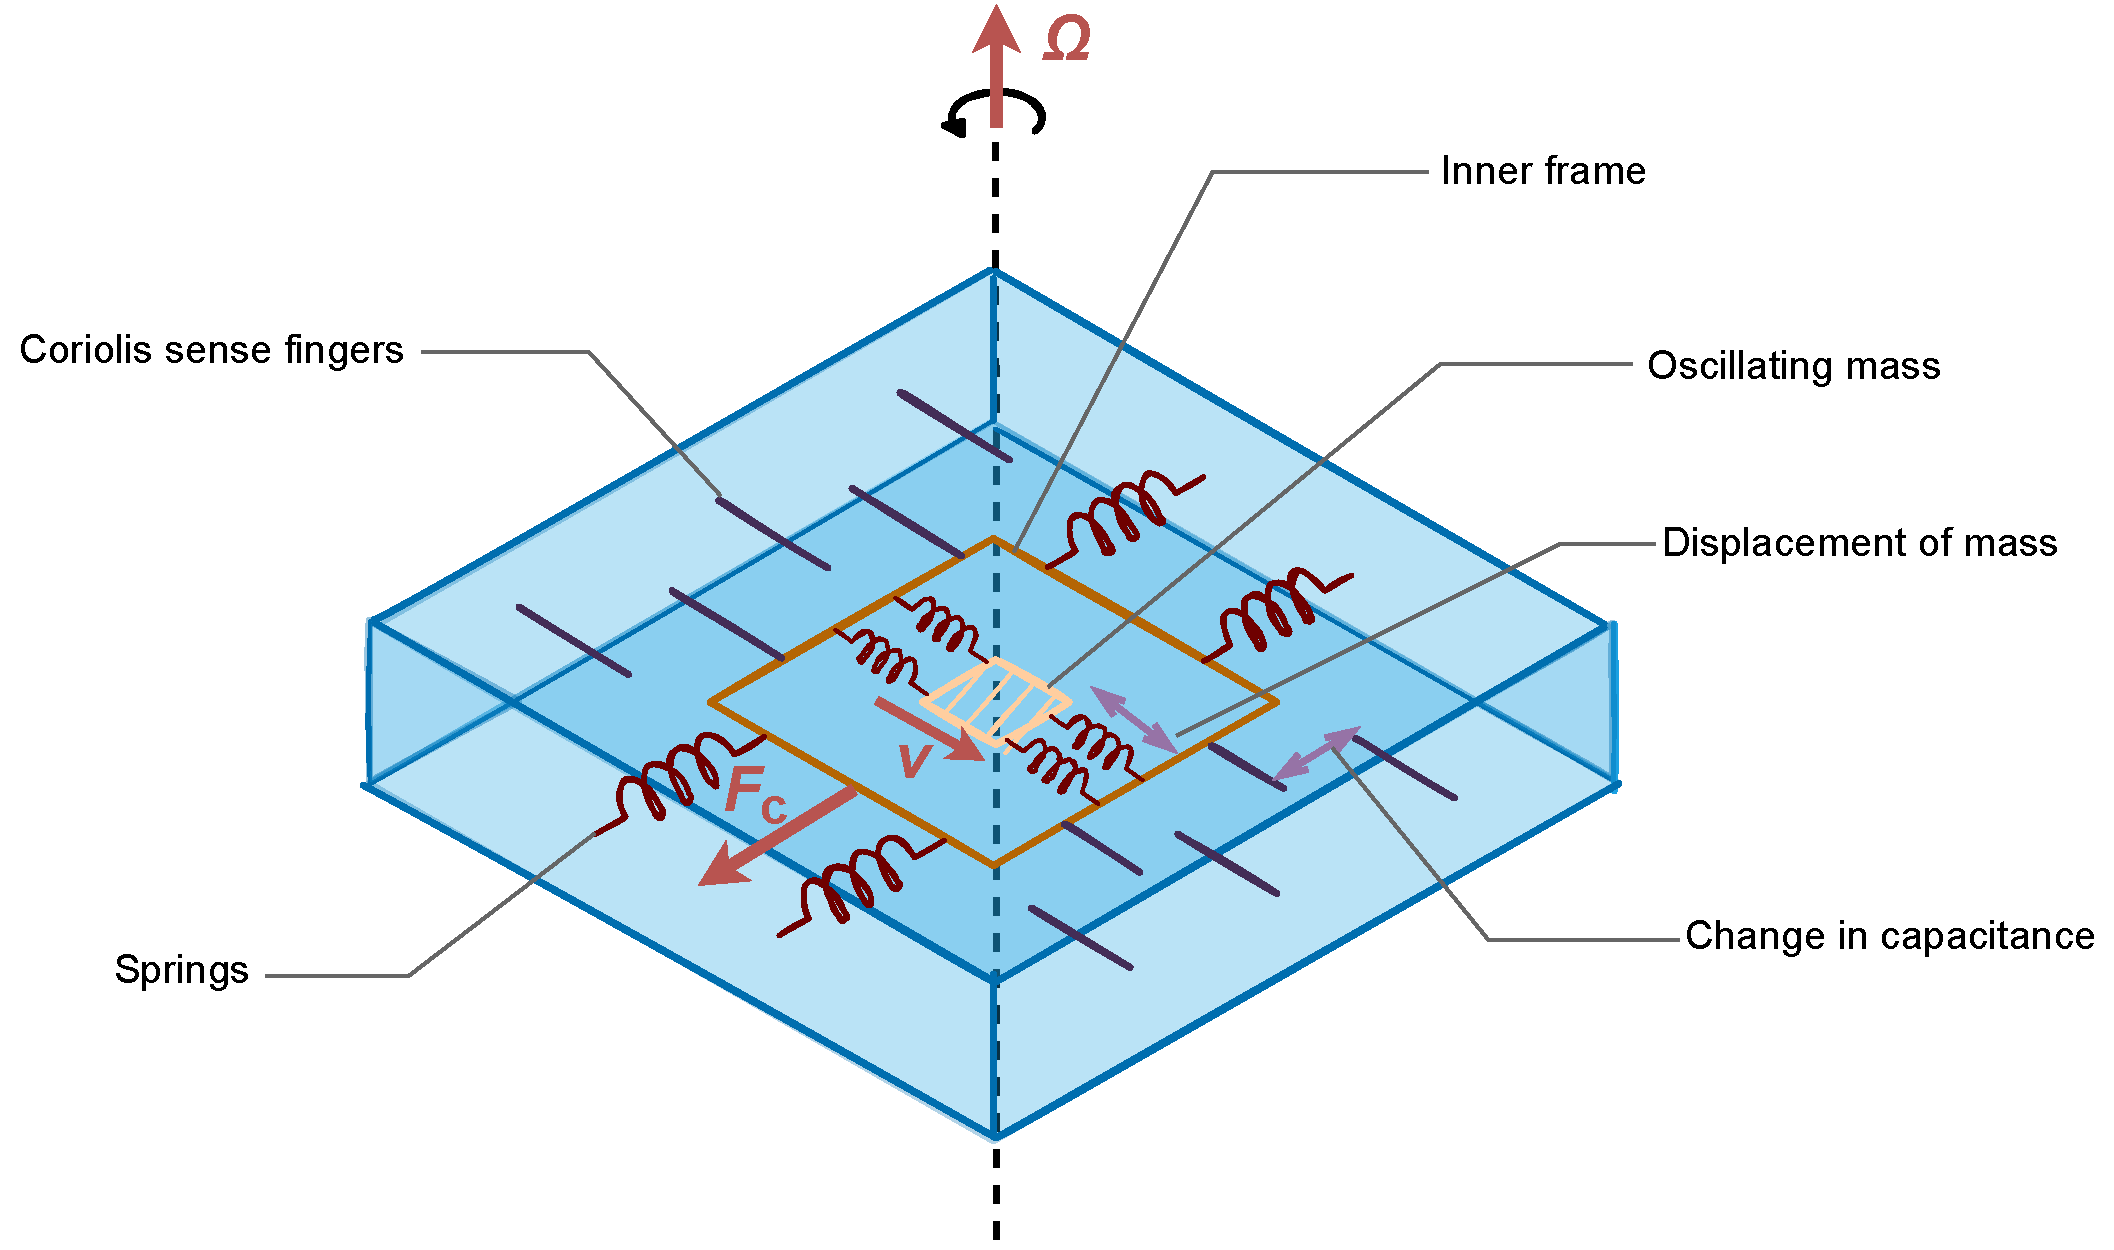
\includegraphics[width=.8\textwidth]{figures/gyroscope.drawio.pdf}
    \caption{Principle of a microfabricated gyroscope to sense the rotation of an out-of-plane rotational velocity vector $\boldsymbol{\mathit{\Omega}}$ (author's own work).}
    \label{fig:gyroscope}
\end{figure}

A driving circuit causes linear oscillation of the central mass, which can move linearly suspended by springs within an inner frame. This frame can move linearly in an orthogonal direction, again suspended by springs. Rotation of the whole sensor around its height axis leads to a lateral displacement of the inner frame, resulting in a change in capacitance between the so-called Coriolis sense fingers. 

The sketch illustrates the situation for a counter-clockwise rotation ($\boldsymbol{\mathit{\Omega}}$ vector upward). When the mass moves to the front right ($\boldsymbol{v}$), the Coriolis force ($\boldsymbol{F}_\mathrm{c}$)  pushes the inner frame to the front left. Upon reversal of the linear movement (mass moves to the back left), the Coriolis force points in the other direction. 
\subsection{Acceleration Sensor}
\xblackout{Lorem ipsum dolor sit amet, consectetur adipiscing elit, sed do eiusmod tempor incididunt ut labore et dolore magna aliqua. Ut enim ad minim veniam, quis nostrud exercitation ullamco laboris nisi ut aliquip ex ea commodo consequat. Duis aute irure dolor in reprehenderit in voluptate velit esse cillum dolore eu fugiat nulla pariatur. Excepteur sint occaecat cupidatat non proident, sunt in culpa qui officia deserunt mollit anim id est laborum.

Lorem ipsum dolor sit amet, consectetur adipiscing elit, sed do eiusmod tempor incididunt ut labore et dolore magna aliqua. Ut enim ad minim veniam, quis nostrud exercitation ullamco laboris nisi ut aliquip ex ea commodo consequat. Duis aute irure dolor in reprehenderit in voluptate velit esse cillum dolore eu fugiat nulla pariatur. Excepteur sint occaecat cupidatat non proident, sunt in culpa qui officia deserunt mollit anim id est laborum. Lorem ipsum dolor sit amet, consectetur adipiscing elit, sed do eiusmod tempor incididunt ut labore et dolore magna aliqua. Ut enim ad minim veniam, quis nostrud exercitation ullamco laboris nisi ut aliquip ex ea commodo consequat. Duis aute irure dolor in reprehenderit in voluptate velit esse cillum dolore eu fugiat nulla pariatur. Excepteur sint occaecat cupidatat non proident, sunt in culpa qui officia deserunt mollit anim id est laborum.}


\begin{figure}[h]
    \centering
    
\includegraphics[width=.6\textwidth]{figures/empty.drawio.pdf}
    \caption{Principle of a microfabricated, capacitive accelerometer to sense the in-plane acceleration (author's own work).}
    \label{fig:gyroscope}
\end{figure}

\clearpage


\section{Methods}
All measurements used the BHI260AP of an Arduino Nicla Sense Board ME connected via USB to a battery-powered notebook acting both as a power supply and data logger. The board was programmed using the Arduino IDE with the \texttt{Arduino\_BHY2} library version 1.5 (Bosch Sensortec). PuTTY (Simon Tatham) was the serial terminal software to log the data.

The Arduino program read the sensors using the virtual sensors \texttt{SENSOR\_ID\_ACC\_PASS} for the acceleration sensors and \texttt{SENSOR\_ID\_GYRO\_PASS} for the gyroscope in the BHI260AP each \SI{100}{\milli\second} resulting in an acquisition rate of \SI{10}{\hertz}. The sensitivity of the acceleration sensor was \SI{417.5}{\LSB\per\metre\square\second} (the default 8$g$ range) and \SI{16.4}{\LSB\per\degree\second} for the gyroscope \cite{BHI260}.

The merry-go-round on a children playground (\censor{Lorem ipsum dolor sit amet}, Freiburg) was spun manually with the Nicla Sense Board ME positioned stably on the notebook, which was placed on the merry-go-round. The distance from the center of rotation to the sensor was $r=0.7$ and \SI{1.0}{\metre}. The rotation was clockwise. The $y$-axis of the board pointed radially to the center, and the $x$-axis opposite to the tangential direction resulting in the $z$-direction pointing upwards (Figure~\ref{fig:setup}).

The measurements for Task~1 were recorded at approximately \SI{29}{\celsius} (indoor). The recordings of Task~2 with the merry-go-round were at approximately \SI{16}{\celsius}.

\vspace{3em}

\begin{figure}[h]
\centering
    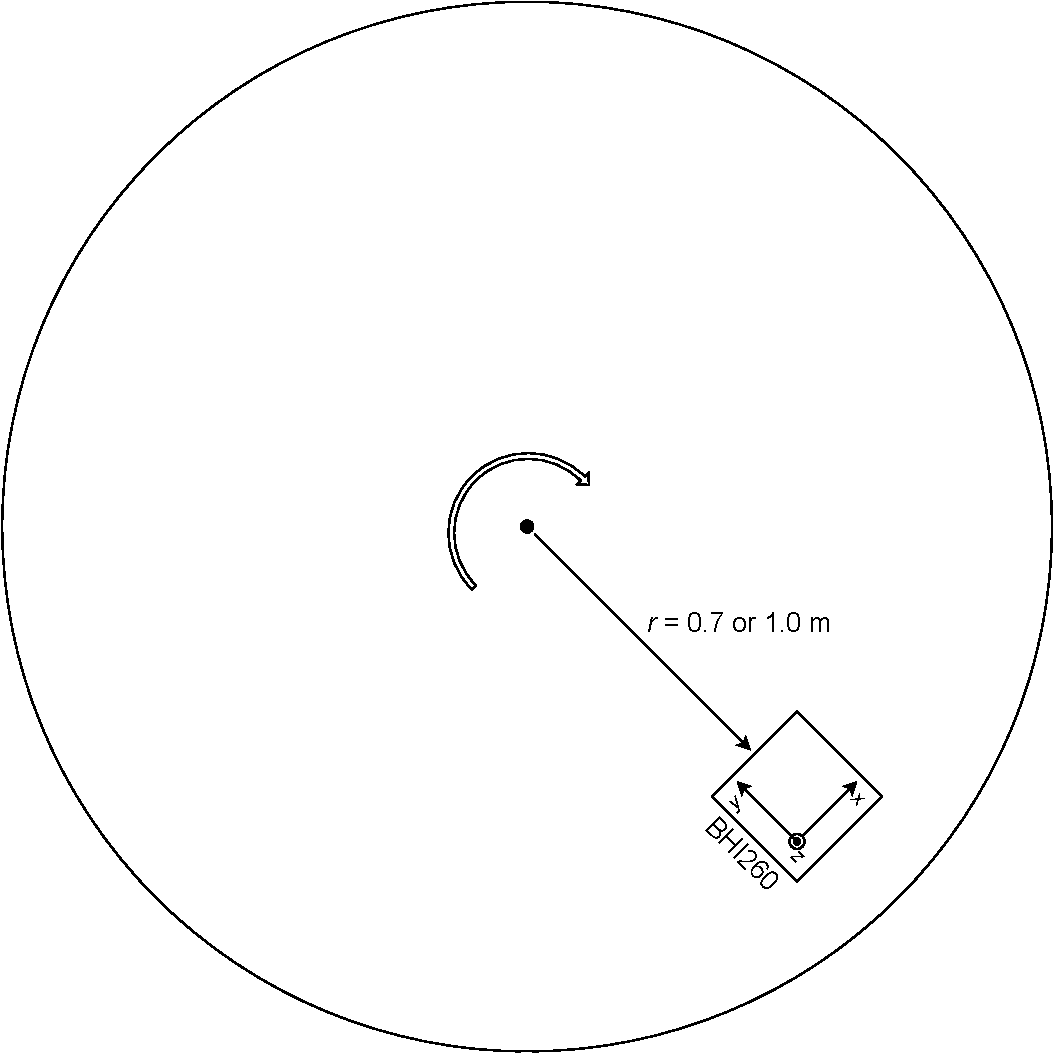
\includegraphics[width=.6\textwidth]{figures/merry-go-round.drawio.pdf}
    \caption{Setup of the merry-go-round measurement (Task~2): the sensor was placed with its $z$-axis pointing upward resulting in negative readings of the rotational velocity for clockwise rotation. The $y$-axis pointed to the center.}
    \label{fig:setup}
\end{figure}

\clearpage

\section{Results and Discussion}

\subsection*{Task 1}

The first task addresses the performance of the gyroscope. Critical aspects are the offset (sensor reading at rest) and the noise level. The Nicla Sense ME Board was placed flat on a steady table and the rotation velocity was recorded. Figure~\ref{fig:gyro_raw} provides an overview on the 1,000 samples in each direction. No drift or offset is visible. No pattern affecting all three directions is noticeable. The obtained values are in the range of the quantization (1~LSB corresponds to \SI{0.06}{\degree\per\second}).

\begin{figure}[h]
    \centering
    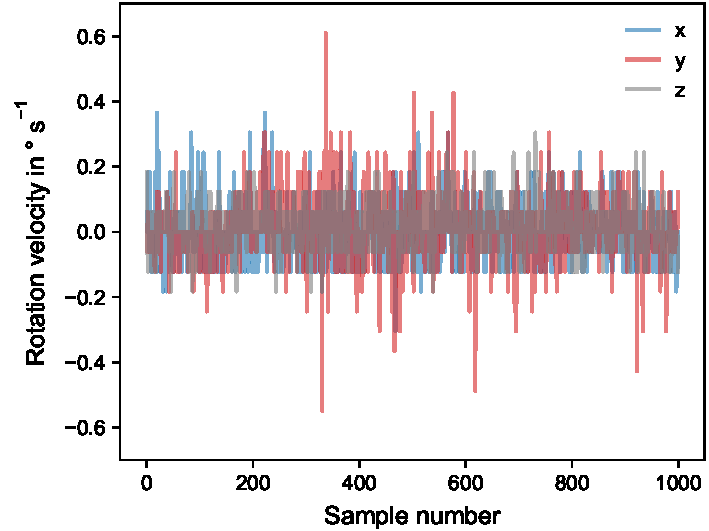
\includegraphics[width=.6\textwidth]{plots/gyro_raw.pdf}
    \caption{Gyroscope readings at rest, the noise level is in the range of the quantification with no clear difference between the three directions. The measurement rate is \SI{10}{\hertz}.}
    \label{fig:gyro_raw}
\end{figure}

\begin{table}[h]
    \begin{tabular}{lS[table-format=1.3]S[table-format=1.3]}\hline \vspace{-1em}  \\ 
    Direction & {Mean value $\bar{\mathit{\Omega}}$ (offset) in \si{\degree\per\second}} &  {Standard deviation $\sigma_\Omega$ in \si{\degree\per\second}} \\ \hline
    $x$ & -0.003  & 0.087  \\
    $y$ & 0.009  & 0.102  \\ 
    $z$ & 0.014  & 0.066 \\ \hline
    \end{tabular}
    \caption{Summary of the rotation velocity $\mathit{\Omega}$ readings at rest, the number of samples was 1,000 in each direction. Please note the quantization of \SI{0.06}{\degree\per\second} for the individual values.}
    \label{tab:gyro}
\end{table}

Evaluation of the data (Table~\ref{tab:gyro} shows summary of the mean values and corresponding standard deviations) shows a very low offset (less than 1~LSB) and accordingly no significant difference between the directions. Also the standard deviation below 2~LSB suggests a very low noise level. The histograms (Figure~\ref{fig:gyro_hist}A--C) reveal the distribution more clearly. Within the limits due to the quantization, the data allows approximation by a normal distribution. 

The sensors for the rotation rate in $x$- and $y$-direction in the BHI260AP probably use a different setup than for the $z$-direction, which could be based on out-of-plane motion. However, even the histogram with the superimposed distributions (Figure~\ref{fig:gyro_hist}D) shows no difference between the different axes.

\begin{figure}[h]
    \centering
    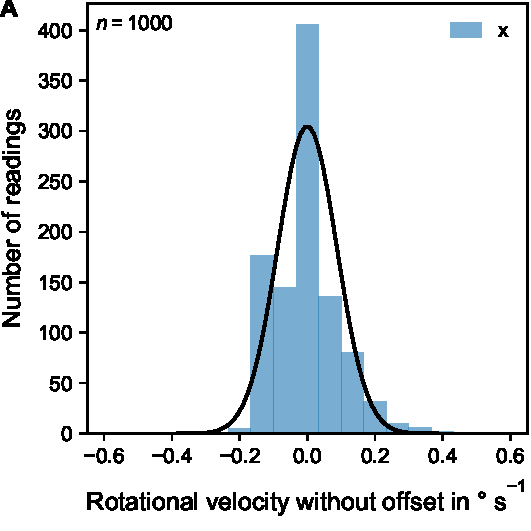
\includegraphics[width=.45\textwidth]{plots/gyro_hist_x.pdf}\hfill
    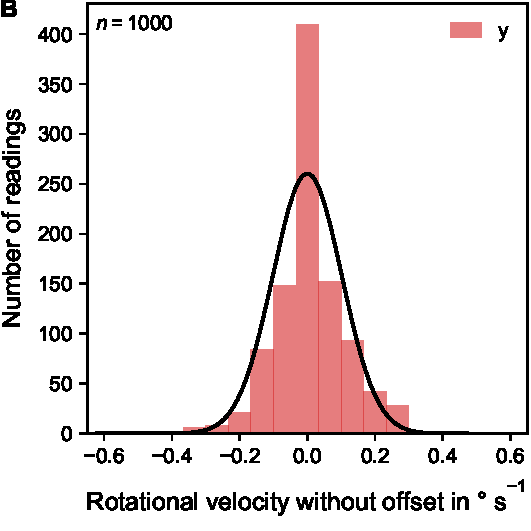
\includegraphics[width=.45\textwidth]{plots/gyro_hist_y.pdf}\vspace{1em}
    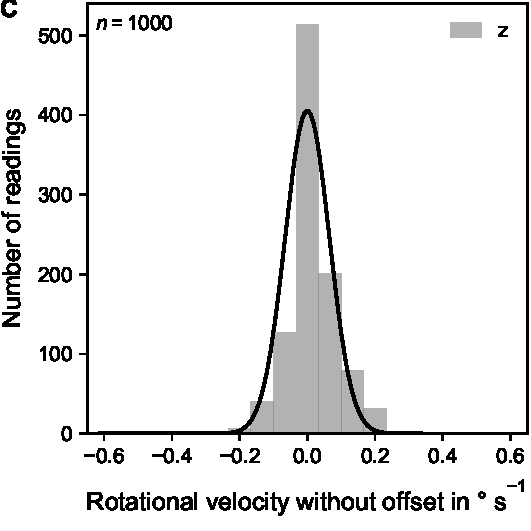
\includegraphics[width=.45\textwidth]{plots/gyro_hist_z.pdf}\hfill
    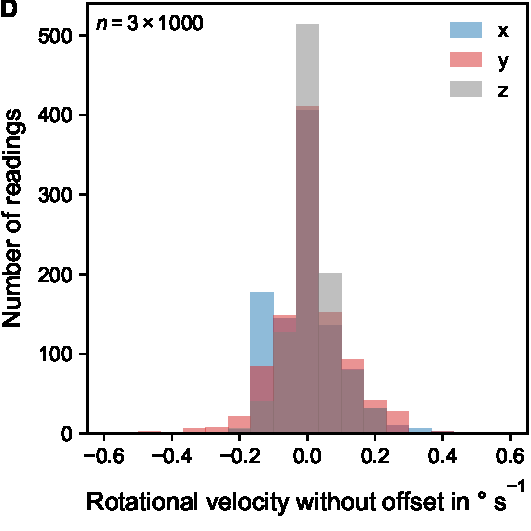
\includegraphics[width=.45\textwidth]{plots/gyro_hist_xyz.pdf}
    \caption{Histograms of the gyroscope reading at rest with subtracted offset: all three directions allow approximation by a normal distribution (A--C), superposition of the three axis (D) show no clear difference between the directions.}
    \label{fig:gyro_hist}
\end{figure}

\clearpage


\subsection*{Task 2}
The measurements on the merry-go-round provided results from the gyroscope and accelerometer. While the overall outcome was the same for the different repetitions, the starting phase strongly depended on how the merry-go-round was pushed and differed for the different trials. During the free ride, the rotational velocity decayed reproducibly, but it was sensitive to movements on the merry-go-round, making this phase also prone to disturbances.

Figure~\ref{fig:gyro_decay} shows the rotational velocity of a typical ride (distance of the sensor from the center was $r=\SI{0.7}{\metre}$). After the maximum, the merry-go-round rode freely with decaying rotational velocity due to friction. Without any external disturbances, the decay was linear.  A linear fit to the undisturbed phase led to a decay of the rotational velocity by \SI{0.8}{\degree\per\square\second}. The coefficient of determination ($R^2$) for the fit was 0.98, confirming the assumption of a linear relationship for the decay.

\vspace{1em}

\begin{figure}[h]
    \centering
    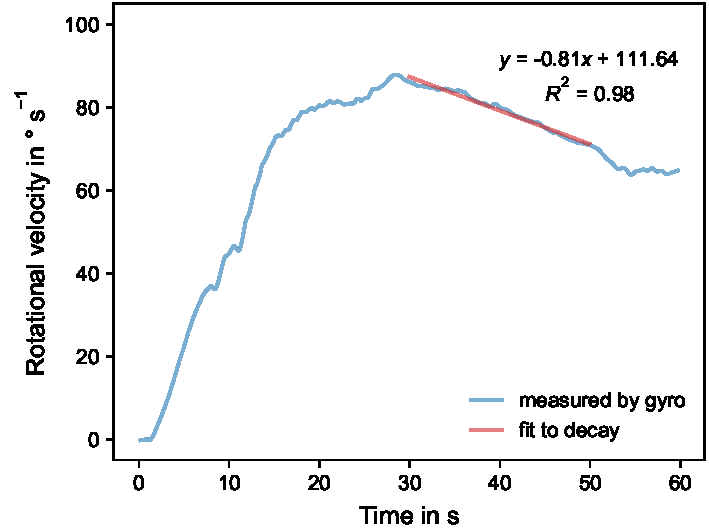
\includegraphics[width=.6\textwidth]{plots/gyro_2_decay.pdf}
    \caption{Rotational velocity measurement with a distance of the sensor from center $r=\SI{0.7}{\metre}$. The sensor values themselves were negative because of the clockwise rotation. Data were smoothed using a running average over 5 samples (\SI{0.5}{\second}).}
    \label{fig:gyro_decay}
\end{figure}

In parallel, the acceleration was measured (Figure~\ref{fig:acc}). The radial acceleration (positive sensor readings) followed the characteristics of the rotational velocity. In contrast, the signals appeared noisy, reflecting the vibrations of the merry-go-round. The tangential acceleration started with negative values during the up-ramping phase but reached positive values before the rotation maximum. 

However, the expected behavior would be that the tangential acceleration changes its sign only at the highest rotational rate, when the propelling of the merry-go-round ends. A possible explanation for this unexpected behavior is a slight misplacement of the Nicla Sense ME Board out of the exact radial axis. In this case, the much larger radial acceleration would superimpose and cause wrong tangential readings, especially for higher rotational velocities.

\begin{figure}[h!]
    \centering
    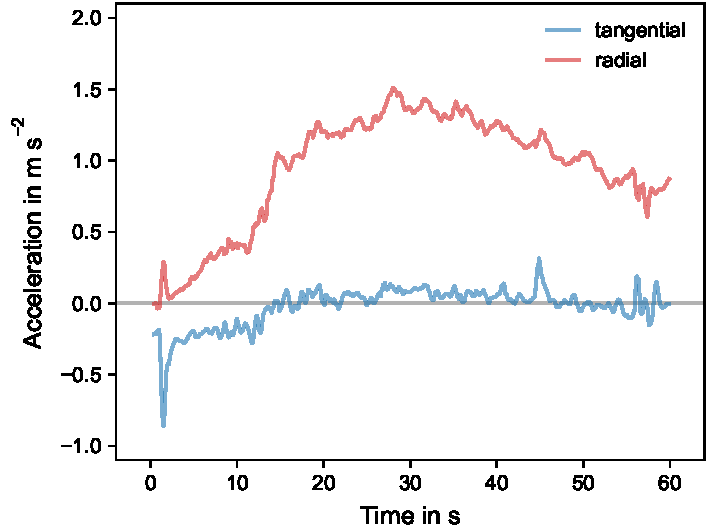
\includegraphics[width=.6\textwidth]{plots/acc_2.pdf}
    \caption{Acceleration measurement with a distance of the sensor from center $r=\SI{0.7}{\metre}$. The plot shows the run from Figure~\ref{fig:gyro_decay}. Data were smoothed using a running average over 5 samples (\SI{0.5}{\second}).}
    \label{fig:acc}
\end{figure}

Figure~\ref{fig:gyro_acc} shows the comparison between the rotational velocity measured by the gyroscope and the values calculated using the relationship of equation~2. For negative acceleration values at the beginning, no calculation was possible because of the square root. Especially for higher rotational speeds, the results match very well.

\begin{figure}[h!]
    \centering
    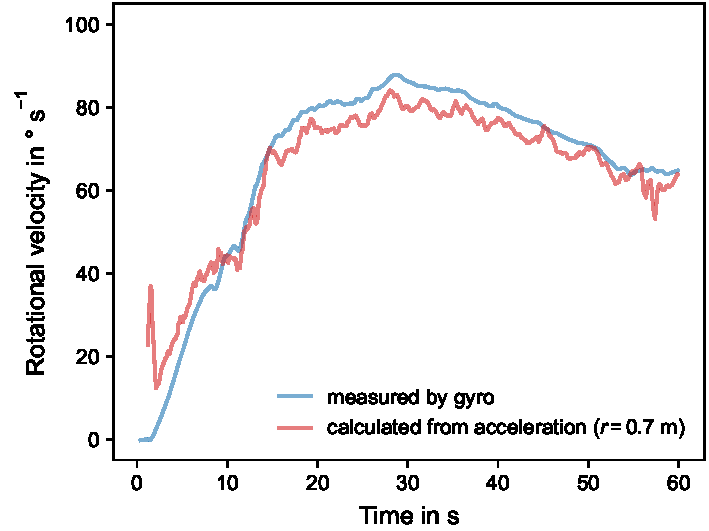
\includegraphics[width=.6\textwidth]{plots/gyro_2.pdf}
    \caption{Rotational velocities with a distance of the sensor from center $r=\SI{0.7}{\metre}$. The plot compares data measured by the gyroscope and values calculated from the radial acceleration. Data were smoothed using a running average over 5 samples (\SI{0.5}{\second}).}
    \label{fig:gyro_acc}
\end{figure}

\clearpage


Table~\ref{tab:gyro_acc} summarizes the evaluation of the measured rotational velocity, the radial acceleration, and therewith calculated rotational velocity at the rotation maximum for the two different distances $r$ between the sensor and the center. Please note that the measured rotational velocity provides information about the direction (negative sign for clockwise rotation when the rotational velocity vector points upwards) in contrast to the value calculated from the radial acceleration. The discrepancy between the values is in both cases below \SI{10}{\percent}. Both, imprecision in $r$ as well as the fluctuations in the acceleration signal can contribute to this discrepancy. 

\vspace{2em}

\begin{table}[h]
    \begin{tabular}{S[table-format=1.1]S[table-format=2.1]S[table-format=1.2]S[table-format=2.1]c}\hline \vspace{-1em}  \\ 
    {$r$ in \si{m}} & {$\mathit{\Omega}_\mathrm{z}$ in \si{\degree\per\second}} &  {$a_\mathrm{y}$ in \si{\metre\per\square\second}} & {$\mathit{\Omega}_\mathrm{calc}$ in \si{\degree\per\second}} & Discrepancy \\ \hline
    0.7 & -87.9  & 1.47 & 83.0 & \SI{5.9}{\percent}  \\
    1.0 & -83.1  & 1.75 & 75.7 & \SI{9.8}{\percent} \\ \hline
    \end{tabular}
    \caption{Comparison of the measured rotational velocity ($\mathit{\Omega}_\mathrm{z}$) to the calculated rotational velocity ($\mathit{\Omega}_\mathrm{calc}$) based on the radial acceleration ($a_\mathrm{y}$) for different distances $r$ between the sensor and the center. The discrepancy describes the relative deviation between the measured and calculated rotational velocity.}
    \label{tab:gyro_acc}
\end{table}


\section{Summary}
Characterization of the gyroscope showed very low offset and noise, both in the range of the LSB. No differences between the three axes were observed. During merry-go-round rides, measurements with the gyroscope and the accelerometer provided realistic results for the rotational velocity, decay of the rotation due to friction, and radial acceleration. Calculating the rotational velocity from the centripetal acceleration lead to values matching well the results from the gyroscope.


% BibTeX or Biber would be better options, with just 2 reference the "raw" approach is fine for such a report
\begin{thebibliography}{------}
 
\bibitem[1]{labManual} J. Kieninger, S.\,J. Rupitsch, \textit{Sensors Lab Course}. University Freiburg. Winter term 2022/23.

\bibitem[2]{BHI260} \textit{BHI260AP Datasheet}, Bosch Sensortec, BST-BHI260AP-DS000-02, rev. 1.1, 15-Apr-2021.

\end{thebibliography}


\end{document}
